The model parameters and their variances are estimated using a combination of static experimental data and dynamic responses obtained under small-perturbation conditions. Subsequently, the resulting model is validated against the dynamic response of the full nonlinear model.

\subsection{Aerodynamic coefficients and friction}
Aerodynamic coefficients and friction parameters are accurately estimated
through a least-squares estimation approach, as depicted in Fig.-\ref{fig::CT}
and Fig.-\ref{fig::CD}. The experimental setup, shown in
Fig.-\ref{fig::expt_setup}, records the total moment at the base, which
encompasses both aerodynamic moments and BLDC motor friction. It's worth noting
that the moment data exhibits greater variability than the model due to
unmodeled aerodynamic effects, such as aerodynamic flutter.
%===

\begin{minipage}{0.49\textwidth}
\begin{figure}[H]
    \centering
    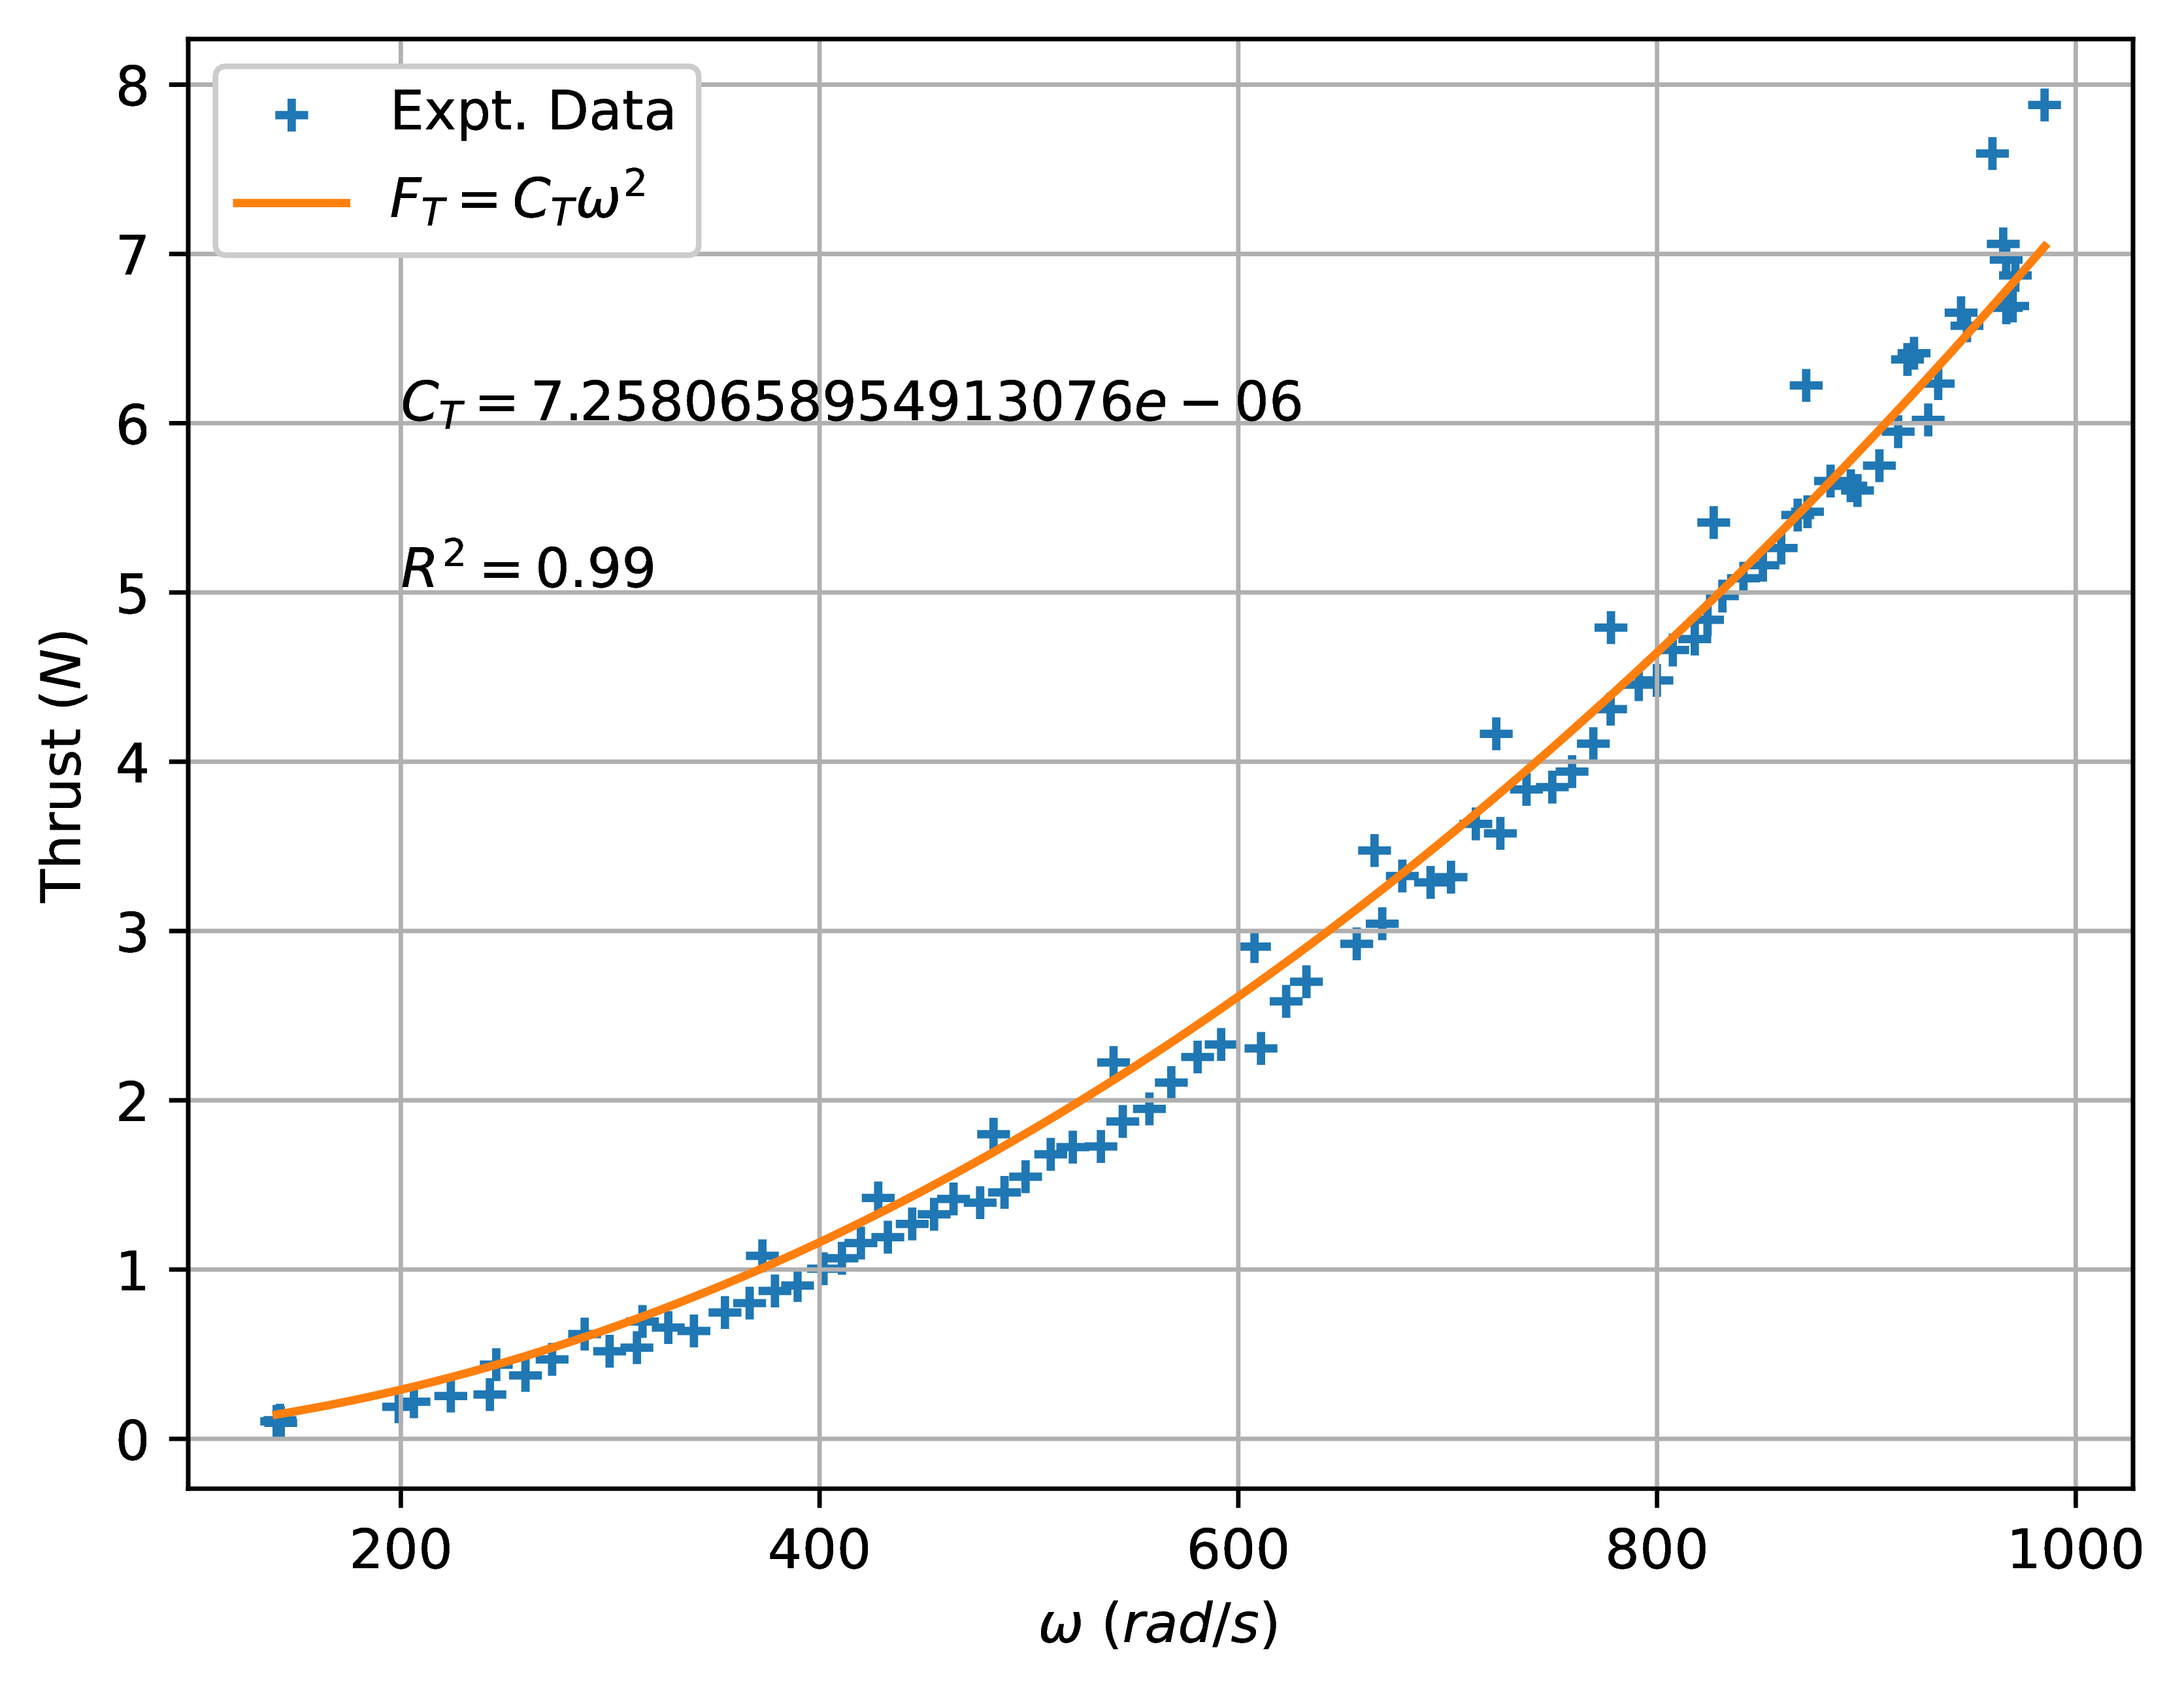
\includegraphics[width = \textwidth]{Part2/figs/3_figs/aero/Thrust_curve.png}
\caption{$C_T$ estimation}
\label{fig::CT}
\end{figure}
\end{minipage}
%===
\begin{minipage}{0.49\textwidth}
\begin{figure}[H]
    \centering
    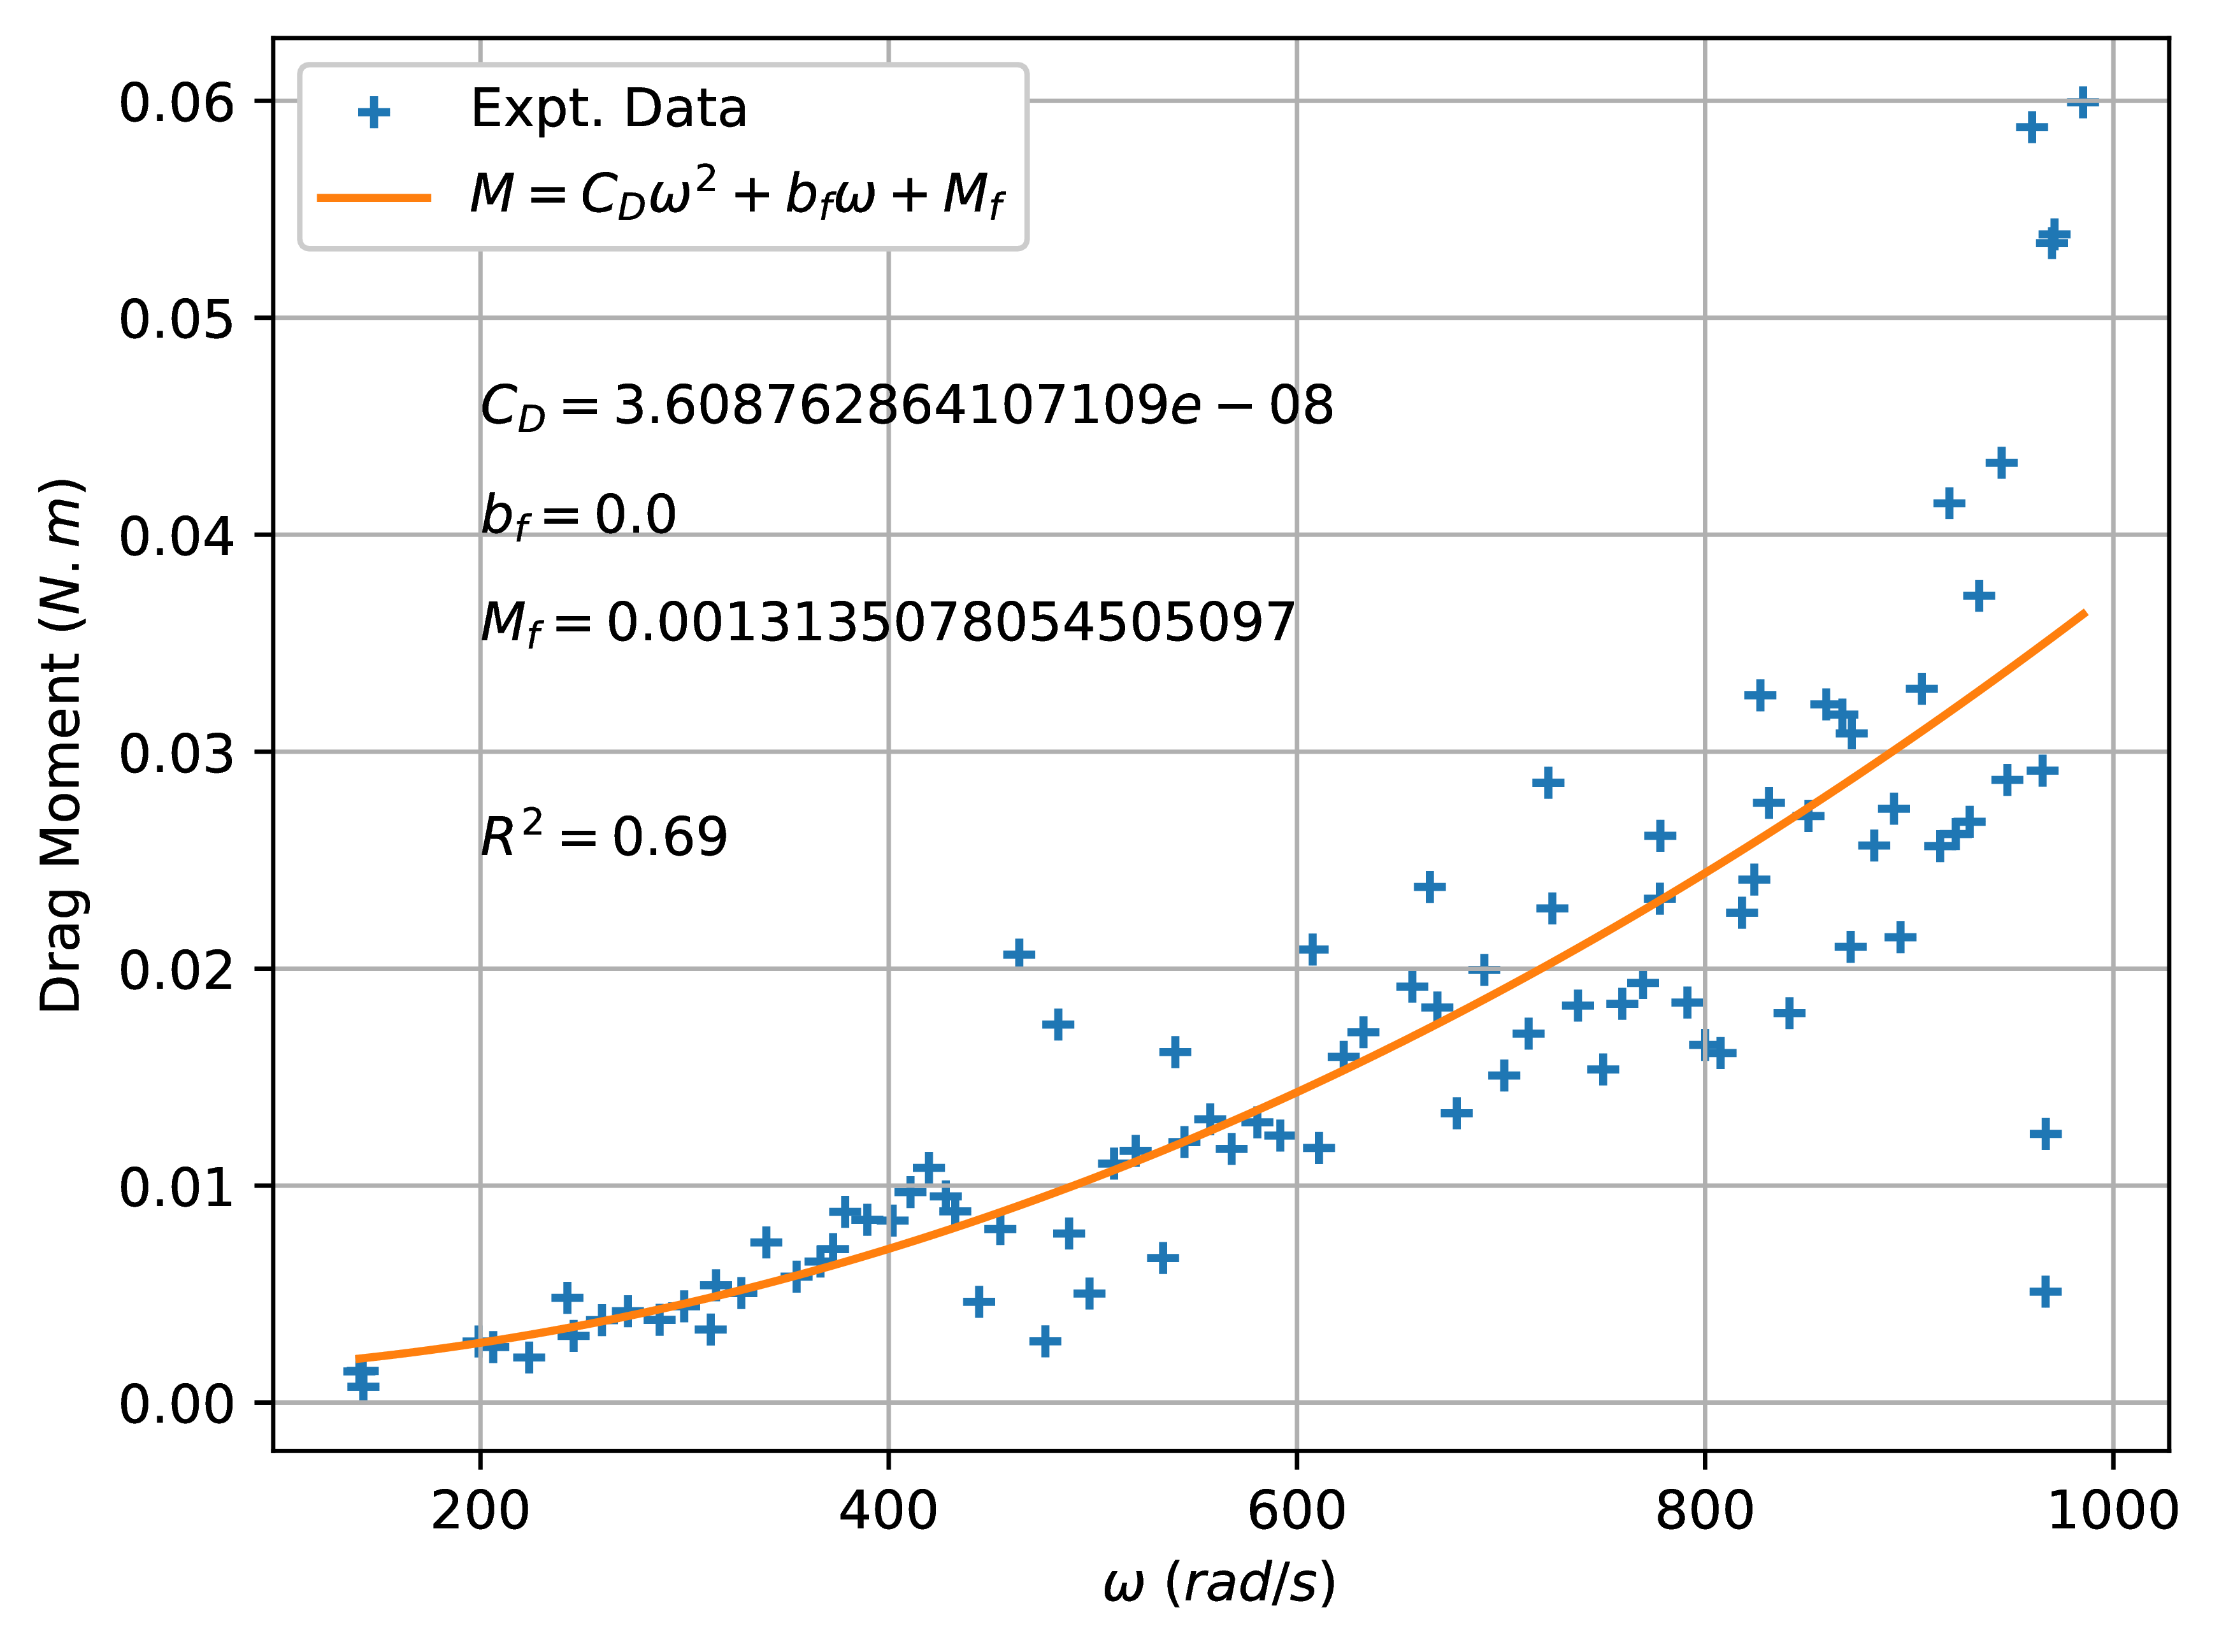
\includegraphics[width = \textwidth]{Part2/figs/3_figs/aero/Drag_curve.png}
    \caption{$C_D$ estimation}
    \label{fig::CD}
\end{figure}
\end{minipage}

%===
\subsection{Linearized model identification and parameter estimation}

The system's response to a Sum-of-Sinusoids signal with a frequency of $250$ Hz and an amplitude of $50 \mu s$ (PWM), encompassing $299$ frequencies within the range of $[0.01, 30]$ Hz, is utilized for identifying first-order model parameters. The selection of this frequency range is based on prior efforts aimed at capturing the system's first-order dynamics with small signal excitations, constrained by the first mode of structural vibration of the fixture \cite{charla2022enhancing}. Table-\ref{tab::nom_in} provides the nominal inputs alongside their corresponding RPM values and validation outcomes. To verify the identified models, their performance is evaluated against the response to a chirp signal with the same frequency range and sampling rate.

The static gain and cutoff frequencies are graphed with respect to the nominal inputs. Parameters linking them to the nominal inputs are estimated using the least-squares method.

The plot of $V_{in}$ and $K$ demonstrates the validity of their relationship when accounting for $V_{in}$ variation, expressed as:
%===
\begin{align}
    K &= V_{in} (1 + \delta v)
\end{align}
%===
\begin{multicols}{2}
 \begin{figure}[H]
    \centering
    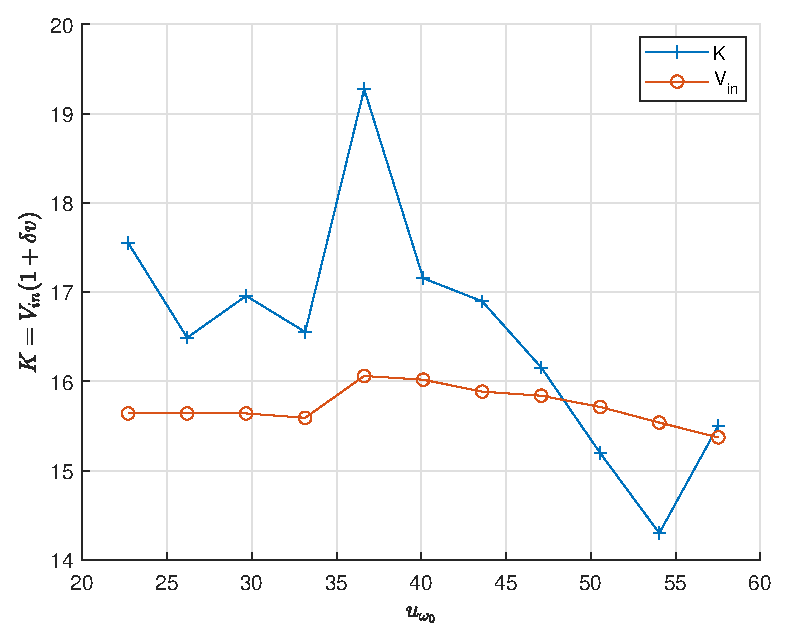
\includegraphics[width = 0.49\textwidth]{Part2/figs/3_figs/small_perturbation/K-Vin.eps}
    \caption{Static gain and Voltage input}
\end{figure}
%===
\begin{figure}[H]
    \centering
    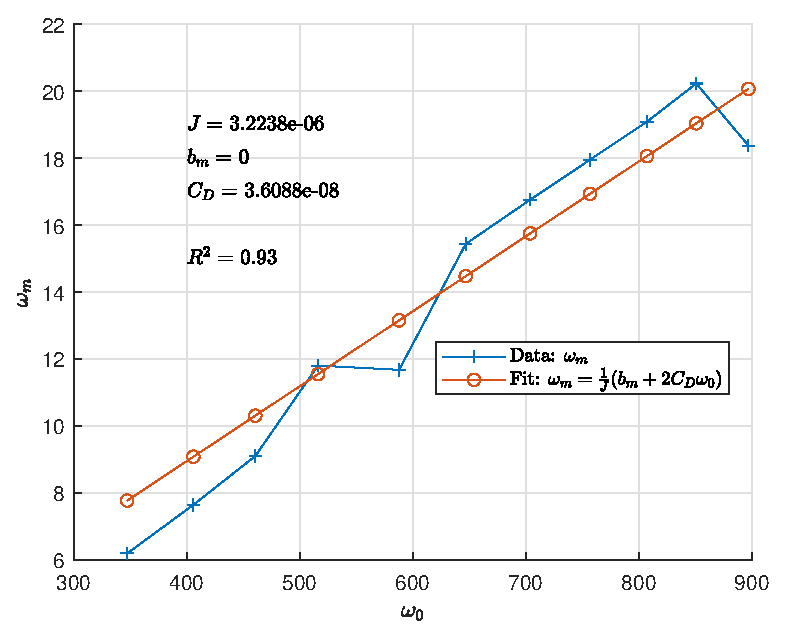
\includegraphics[width = 0.49\textwidth]{Part2/figs/3_figs/small_perturbation/omega_fit.eps}
    \caption{Cut-off frequency}
\end{figure}
\end{multicols}
%===
Furthermore, based on the static gain values, we can estimate the maximum magnitude of $\abs{\delta v}$ as follows:
%===
\begin{align}
    \abs{\delta v}_{max} = \frac{ \max\lr{\abs{K - V_{in}}}}{V_{in}} = 0.2
\end{align}
%===
\begin{table}[h]
    \centering
    \caption{\centering Summary of parameter estimates from static and small-perturbation experiments}
    \label{tab::parm_ests}
    \begin{tabular}{c r l c}
        \hline \hline
        Parameter & Value & & $\sigma$           \\ \hline \hline
        $C_T$ & $7.2581 \times 10^{-06}$ & $N/(rad/s)^2$   & $4.4522 \times 10^{-8}$ \\
        $C_D$ & $3.6088 \times 10^{-08}$ & $N.m/(rad/s)^2$ & $1.3964 \times 10^{-9}$ \\
        $b_m$ & $0.0$                    & $N.m/(rad/s)$   & $4.6003 \times 10^{-6}$  \\
        $M_f$ & $1.3135 \times 10^{-3}$  & $N.m$           & $4.5277 \times 10^{-3}$ \\
        $J$   & $3.2238 \times 10^{-6}$   & $Kg.m^2$        & $7.0053 \times 10^{-6}$ \\
        \hline \hline
    \end{tabular}
    \begin{flushleft}
        ($\sigma - $ Standard deviation of the estimates)
    \end{flushleft}
\end{table}

%===
\subsection{Validation}
The non-linear model is simulated using a square wave and a chirp input
covering the entire operating range in terms of amplitude, assuming $\delta v =
0$. The simulation results are compared with experimental data using the
same input data in Fig.-\ref{fig::sq_valid} and Fig.-\ref{fig::chirp_valid}.
These figures indicate that the model parameters are estimated with reasonable
accuracy. Any discrepancies between the simulation and experimental data can
primarily be attributed to non-zero $\delta v$ and sensor noise.
%===

\begin{minipage}{0.49\textwidth}
 \begin{figure}[H]
    \centering
    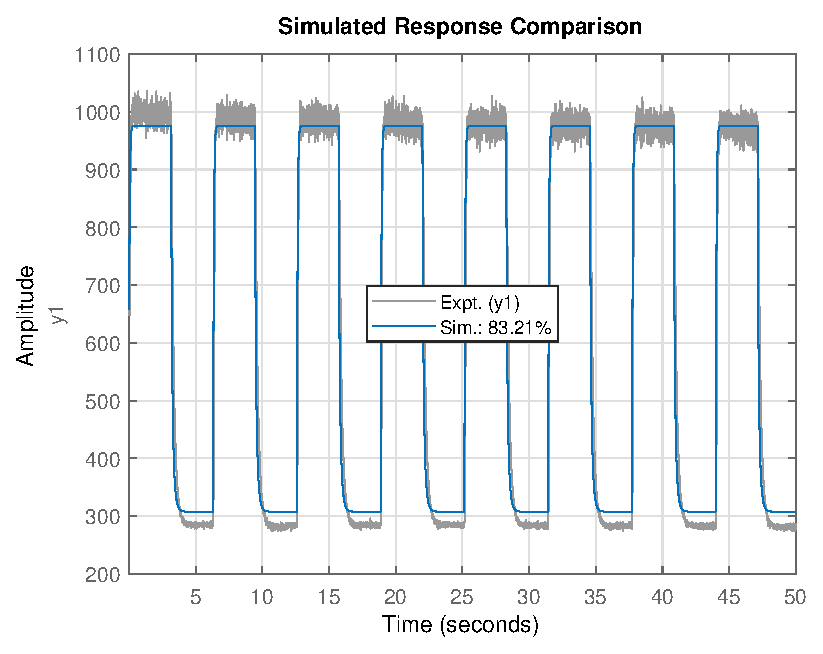
\includegraphics[width = \textwidth]{Part2/figs/3_figs/nl_valid/square_validation.eps}
    \caption{Square Wave Input Response}
    \label{fig::sq_valid}
\end{figure}
\end{minipage}
\begin{minipage}{0.49\textwidth}
\begin{figure}[H]
    \centering
    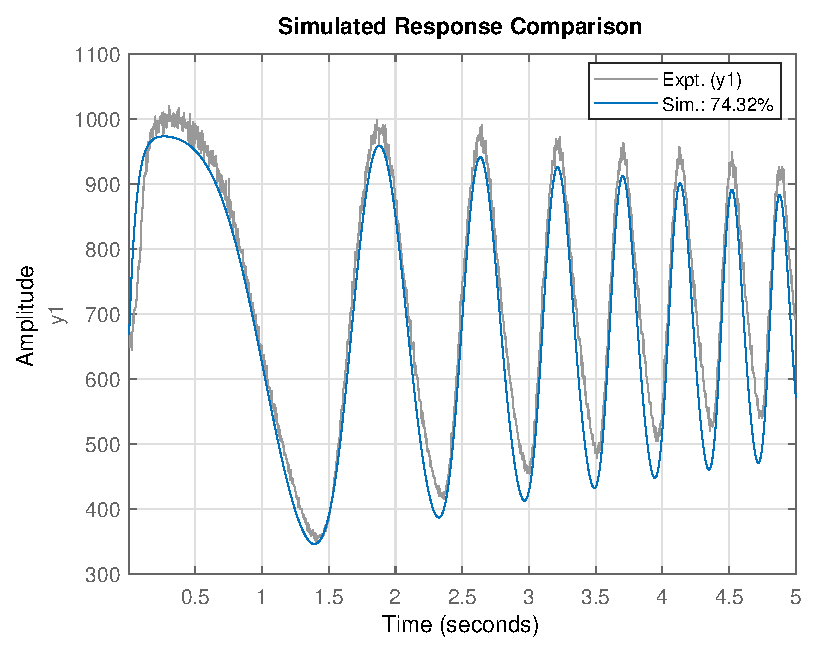
\includegraphics[width = \textwidth]{Part2/figs/3_figs/nl_valid/chirp_validation.eps}
    \caption{Chirp Input Response}
    \label{fig::chirp_valid}
\end{figure}
\end{minipage}

%===
